\chapter{Apache Spark}

In this thesis, Apache Spark are the main tool to do data processing. This chapter mainly about distributed computing basics and sparks.\\

Apache Spark is an open source cluster computing framework with the features of fast, easy to use and wide supported. Originated at the UC Berkeley AMPLab in 2009 and later contributed to the Apache Software Foundation in 2010, Spark are designed to support wider class of applications than MapReduce, while retaining its properties like fault tolerance, data locality and scalability \cite{1_ryza_laserson_owen_wills}.\\


Spark is a flexible operational framework, Spark Streaming is designed for data stream processing, Spark SQL is good at interactive analysis, MLLib is a good machine learning applications, so Spark can become a versatile big data computing platform\cite{apache_spark}. Spark allows users to load data to the cluster memory, and do repeated operation on these data many times, which makes it very suitable for machine learning.

\section{Compare with Hadoop MapReduce}

The birth of Hadoop MapReduce can be traced back to over 10 years ago, the Google File System paper\cite{ghemawat2003google}, and MapReduce: Simplified Data Processing on Large Clusters\cite{dean2008mapreduce}. Hadoop was first released in April 2006. In December 2011, version 1.0.0 was released. Version 2.X was first released in August 2013. The latest version by June 24, 2016 is 2.7.2.\cite{2_wadkarsiddalingaiah}.\\


Hadoop is not good at iterative computations that need to run the same Mapper and Reducer multiple times, with output from the reducer as the input to the mapper of the next stage (like machine learning). As shown in Figure~\ref{fg:hadoop}, while Hadoop MapReduce is processing computing, it need to store intermediate data into HDFS, which causes extensive data movement and duplication across the network and file system. As a result, HDFS I/O is often the bottleneck of this system.\cite{2_wadkarsiddalingaiah}.
\begin{figure}[h]
	\centering
	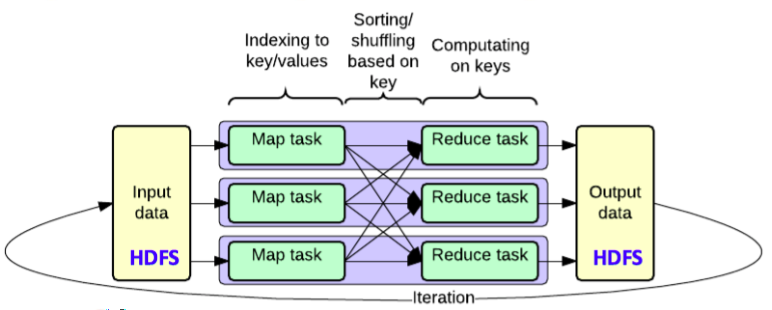
\includegraphics[width=0.9\textwidth]{hadoopcycle}
	\caption{Data cycle in Hadoop MapReduce}
	\label{fg:hadoop}
\end{figure}


\clearpage
From the above description, MapReduce don’t have efficient data sharing method. Spark solve this problem using In-Memory data processing and sharing\cite{apache_spark}. As shown in Figure~\ref{fg:spark}, Spark is based on the in-memory framework. While computing, those intermediate data is temporarily stored in memory, which greatly speed up the execution. Especially for those applications that needs iterations.

\begin{figure}[h]
	\centering
	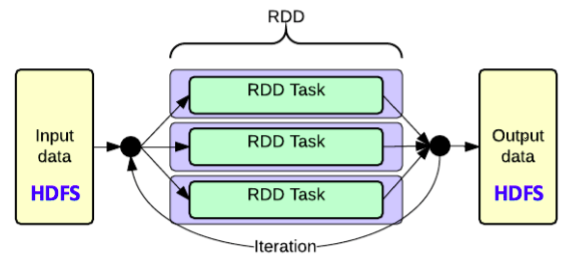
\includegraphics[width=0.8\textwidth]{sparkcycle}
	\caption{Data cycle in Hadoop MapReduce}
	\label{fg:spark}
\end{figure}


The result in contest also prove this theory. In the Daytona GraySort contest for 2014, Apache Spark wins the first price\cite{3_xin_2014}. Results can be find in table~\ref{tb:hadoop_vs_spark}. Spark sorted the same data 3X faster using 10X fewer machines.
\begin{table}[h]
	\centering
	\resizebox{\textwidth}{!}{%
		\begin{tabular}{|l|c|c|c|}
			\hline
			& \textbf{Hadoop World Record} & \textbf{Spark 100 TB} & \textbf{Spark 1 PB} \\ \hline
			\textbf{Data Size} & 102.5 TB & 100 TB & 1000 TB \\ \hline
			\textbf{Elapsed Time} & 72 mins & 23 mins & 234 mins \\ \hline
			\textbf{\# Nodes} & 2100 & 206 & 190 \\ \hline
			\textbf{\# Coes} & 50400 & 6592 & 6080 \\ \hline
			\textbf{\# Reducers} & 10,000 & 29,000 & 250,000 \\ \hline
			\textbf{Rate} & 1.42 TB/min & 4.27 TB/min & 4.27 TB/min \\ \hline
			\textbf{Rate / node} & 0.67 GB/min & 20.7 GB/min & 22.5 GB/min \\ \hline
			\textbf{Sort Benchmark Daytona Rules} & Yes & Yes & No \\ \hline
			\textbf{Environment} & dedicated data center & EC2 (i2.8xlarge) & EC2 (i2.8xlarge) \\ \hline
		\end{tabular}%
	}
	\caption{Spark TeraSort vs MapReduce\cite{3_xin_2014}}
	\label{tb:hadoop_vs_spark}
\end{table}

However, this design brings a big challenge to Spark’s Fault Tolerance, as once one machine lost, then many data need to be re-computed.

\clearpage
\section{Core Technology in Spark}
Resilient distributed datasets, or RDD, designed based on Matei \cite{zaharia2012resilient}, is one of the core technology in Spark frame. RDD can be regard as a table in database, which can hold any type of data. Spark save data to different partitions RDD \cite{ryza2015advanced}.\\


Every RDD can contain many partitions, a partition is a part of dataset. RDD can rely on each other. The case that each partition of the parent RDD is used by at most one partition of the child RDD is called narrow dependency; while multiple child partitions may depend on one parent partition is called wide dependencies\cite{ryza2015advanced}.
\begin{figure}[h]
	\centering
	\subfigure[Narrow Dependency]{
		\centering
		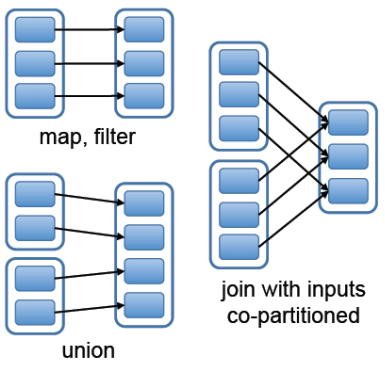
\includegraphics[width=.6\linewidth]{narrowdependencies}
	}
	\subfigure[Wide Denpendency]{
		\centering
		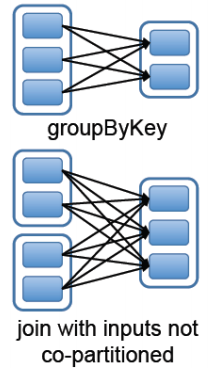
\includegraphics[width=.3\linewidth]{widedependences}
	}
	\caption{Two types of Spark Dependency\cite{zaharia2016architecture}}
\end{figure} 
\clearpage

There are two reasons that why Spark make narrow dependencies out of wide one\cite{zaharia2016architecture},
\begin{enumerate}
	\item Narrow allow for pipelined execution on one cluster node, while wide dependencies must wait for all the parent partitions available.
	\item Fault recover is much easier for narrow dependencies, as it just need to re-compute the lost partitions, and this operation can be done in different nodes. On the other hand, wide dependencies involves many parent partitions.
\end{enumerate}